%\documentclass[11pt]{article}
%\usepackage[utf8]{inputenc}
%\usepackage[spanish]{babel}
%\usepackage[]{graphicx}
%\usepackage{colortbl} %para las tablas
%\usepackage{longtable} %para las tablas
%\usepackage{geometry}
%\geometry{tmargin=3cm,bmargin=3cm,lmargin=3cm,rmargin=2cm}
%
%\begin{document}

%****************************************************************
\subsection{Diagrama de Clases}
				
	\begin{tabular}{|p{5cm}|p{11cm}|}\hline
	{\bf Titulo} & {Diagrama de Clases Usuario}\\
	\hline
	{\bf Descripción} & {El diagrama de clases usuario reúne todas las clases
	relacionadas con la gestión de usuarios en el sistema.\newline
	Explica como se modelo la gestión de usuarios; las clases que interactúan 
	directamente con el usuario	son las guis: GuiAutenticar usada para ingresar
	al sistema, GuiConsultarUsuarios usada para realizar las consultas de usuarios
	para dar soporte al caso de uso modificar usuarios, esta gui es usada por el usuario
	administrador, GuiRegistroModificar es usada para que un usuario se registre
	en el sistema, también para que un usuario registrado pueda modificar sus datos, y
	finalmente para que un usuario administrador pueda modificar estado (activo-desactivo) y
	perfil de un usuario normal. \newline
	La clase que se usa para modelar la entidad Usuario del modelo de datos es precisamente
	la clase usuario, esta clase como se muestra en el diagrama se usa a nivel de gui hacia
	abajo, está también la clase ControladorUsuario que se encarga de realizar las debidas
	verificaciones y de enviar correctamente los datos para las consultas a la clase DaoUsuario 
	que es quien se comunica directamente con la base de datos del sistema.\newline
	Las clases ControladorVentanaPrincipal, DaoArea, Area y FachadaBD son clases que se usan para 
	lograr la gestión de usuarios, las relaciones se muestran en el diagrama.}\\
	\hline
	\end{tabular}\\[.5cm]
		
	\begin{tabular}{|p{3.5cm}|p{4.5cm}|p{2.5cm}|p{4.5cm}|}\hline
	{\bf Creado Por} & {Edgar Andrés Moncada} & {\bf Fecha} & {Abril 25 2011}\\
	\hline
	{\bf Actualizado por} & {Yerminson Gonzalez} & {\bf Fecha} & {Mayo 10 2011}\\
	\hline
	\end{tabular}

	\begin{minipage}[c]{1\linewidth}
	\centering
	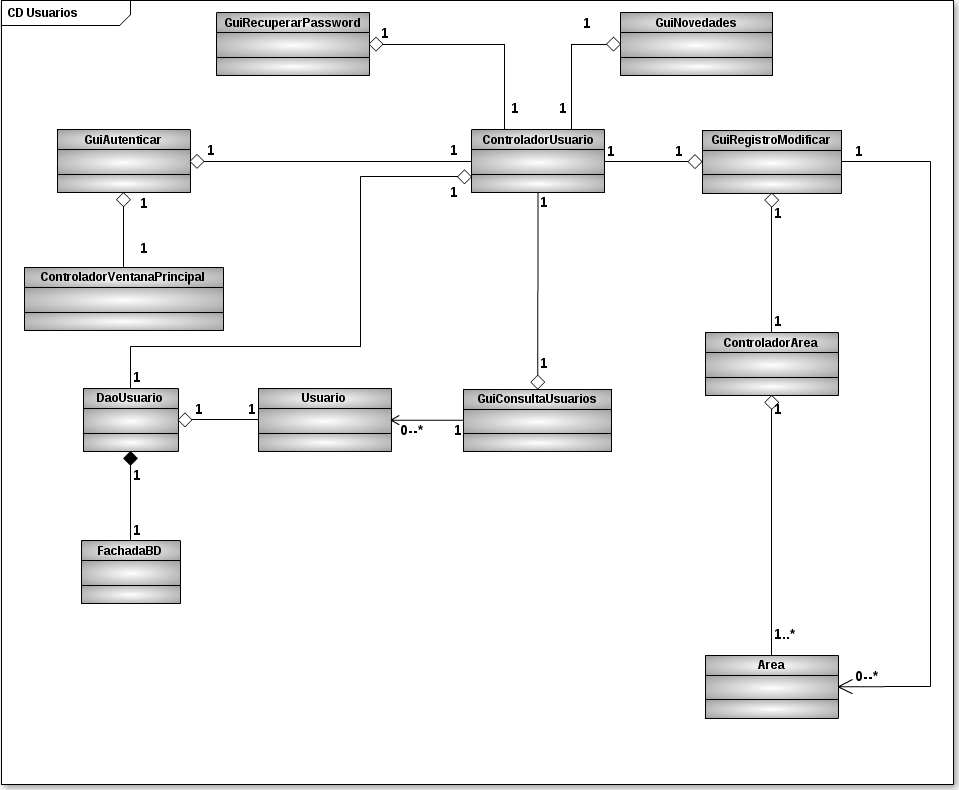
\includegraphics[width=20cm, height=17cm, angle=90]{diagramasClase/DiagramaClases1}
	\end{minipage}
			
	%especificación detallada
	%\documentclass{article}
%
%\usepackage[spanish]{babel}
%\usepackage[utf8]{inputenc}
%\usepackage{geometry}
%\usepackage{graphicx}
%\geometry{tmargin=3cm,bmargin=3cm,lmargin=3cm,rmargin=2cm}
%
%\begin{document}

\setlength{\unitlength}{1cm}
%\begin{picture}(17,21)
%\put(0,0) {\line(1,0){17}}
%\put(0,21) {\line(1,0){17}}
%\put(0,21) {\line(0,-1){21}}
%\put(17,21) {\line(0,-1){21}}
%\end{picture}

\begin{picture}(17,21)
\put(0,2)
{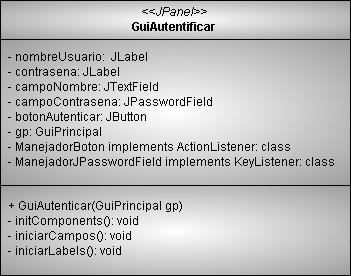
\includegraphics[width=7cm, height=8cm]{DiagramasClase/Usuarios/GuiAutenticar}}
\put(8.5,0)
{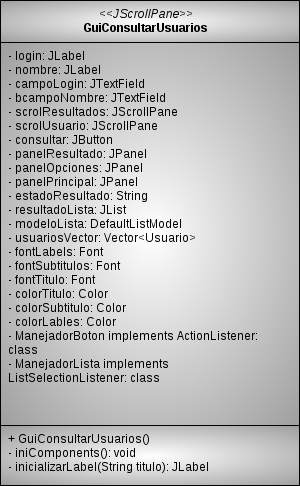
\includegraphics[width=7cm, height=10cm]{DiagramasClase/Usuarios/GuiConsultarUsuarios}}
\put(0,11)
{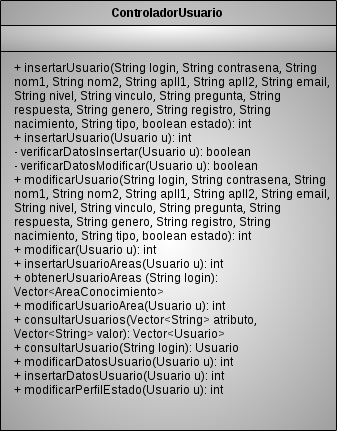
\includegraphics[width=8cm, height=10cm]{DiagramasClase/Usuarios/ControladorUsuario}}
\put(8.5,11)
{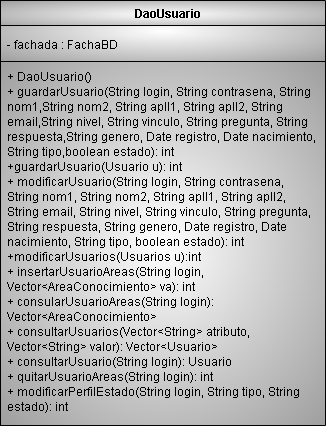
\includegraphics[width=8cm, height=10cm]{DiagramasClase/Usuarios/DaoUsuario}}
\end{picture}

\newpage

\begin{picture}(17,21)
\put(8.5,0)
{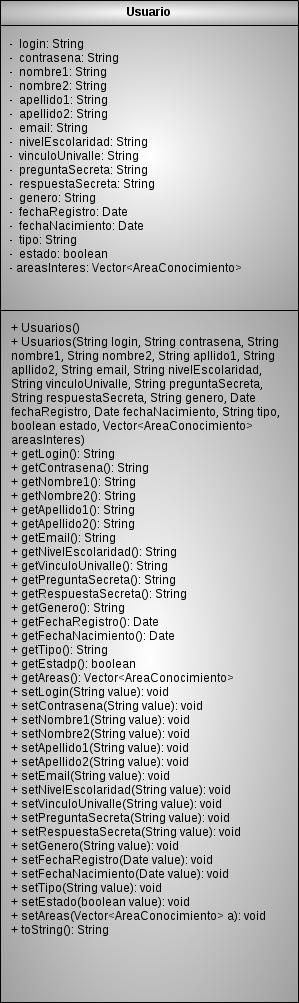
\includegraphics[width=8cm, height=21cm]{DiagramasClase/Usuarios/Usuario}}
\put(0,0)
{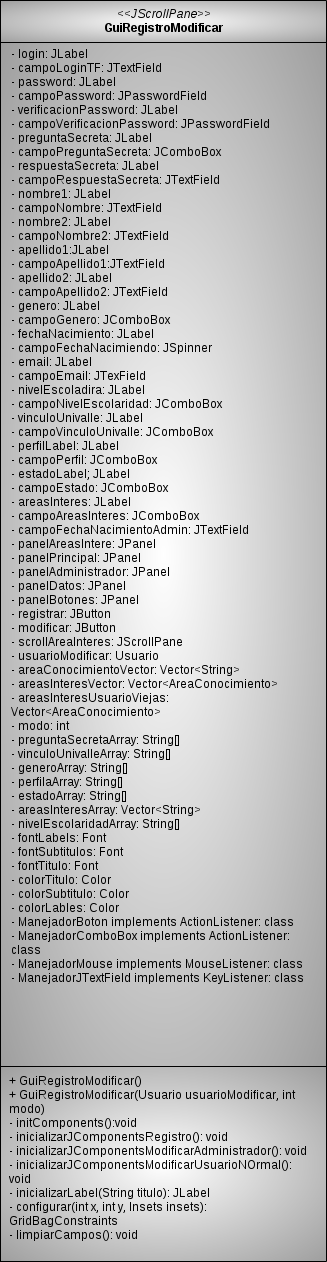
\includegraphics[width=8cm, height=21cm]{DiagramasClase/Usuarios/GuiRegistroModificar}}
\end{picture}

\newpage

\begin{picture}(17,12)
\put(8.5,1)
{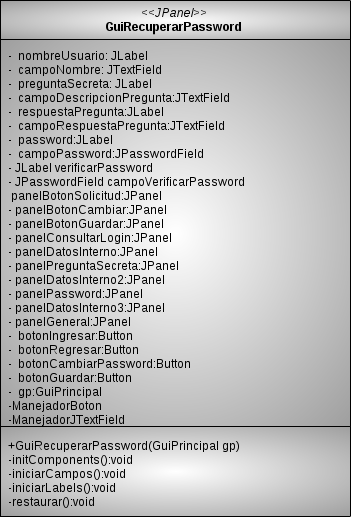
\includegraphics[width=8cm, height=11cm]{DiagramasClase/Usuarios/GuiRecuperarPassword}}
\put(0,4)
{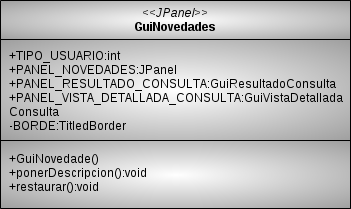
\includegraphics[width=7cm, height=7cm]{DiagramasClase/Usuarios/GuiNovedades}}
\end{picture}
%\begin{minipage}{0.5\textwidth}
%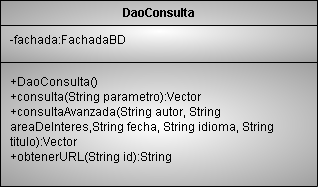
\includegraphics[width=1\textwidth, height=8cm]{DiagramasClase/Consultas/DaoConsulta}
%\end{minipage}

%\end{document}	
	
	%-------------------------------------------------------------------------------	

				
	\begin{tabular}{|p{5cm}|p{11cm}|}\hline
	{\bf Titulo} & {Diagrama de Clases Documento}\\
	\hline
	{\bf Descripción} & {El diagrama de clases documento reúne todas las clases
	relacionadas con la gestión de documentos en el sistema.\newline
	La clase GuiCatalogarModificar es la que permite el registro de nuevos documentos
	en el sistema, Documento modela la entidad documento en el modelo de datos esta clase
	se usa de la gui hacia abajo, la clase ControladorDocumento realiza las verificaciones 
	pertinentes, y envia los valores para realizar consultas y actualizaciones a la clase 
	DaoDocumento que es la encargada de comunicarse directamente con la base de datos del
	sistema.\newline
	Las clases FachadaBD, GuiIngresarArea, GuiIngresarAutor, GuiIngresarTipoMaterial,
	GuiIngresarPalabraClave,ControladorArea, ControladorAutor, ControladorTipoMaterial,
	ControladorPalabraClave, PalabraClave, Autor, y Area son usadas para lograr la gestión de
	documentos.}\\
	\hline
	\end{tabular}\\[.5cm]
	
	\begin{tabular}{|p{3.5cm}|p{4.5cm}|p{2.5cm}|p{4.5cm}|}\hline
	{\bf Creado Por} & {Luis Felipe Vargas} & {\bf Fecha} & {Abril 28 2011}\\
	\hline
	{\bf Actualizado por} & {Edgar Andrés Moncada} & {\bf Fecha} & {Mayo 10 2011}\\
	\hline
	\end{tabular}

	\begin{minipage}[c]{1\linewidth}
	\centering
	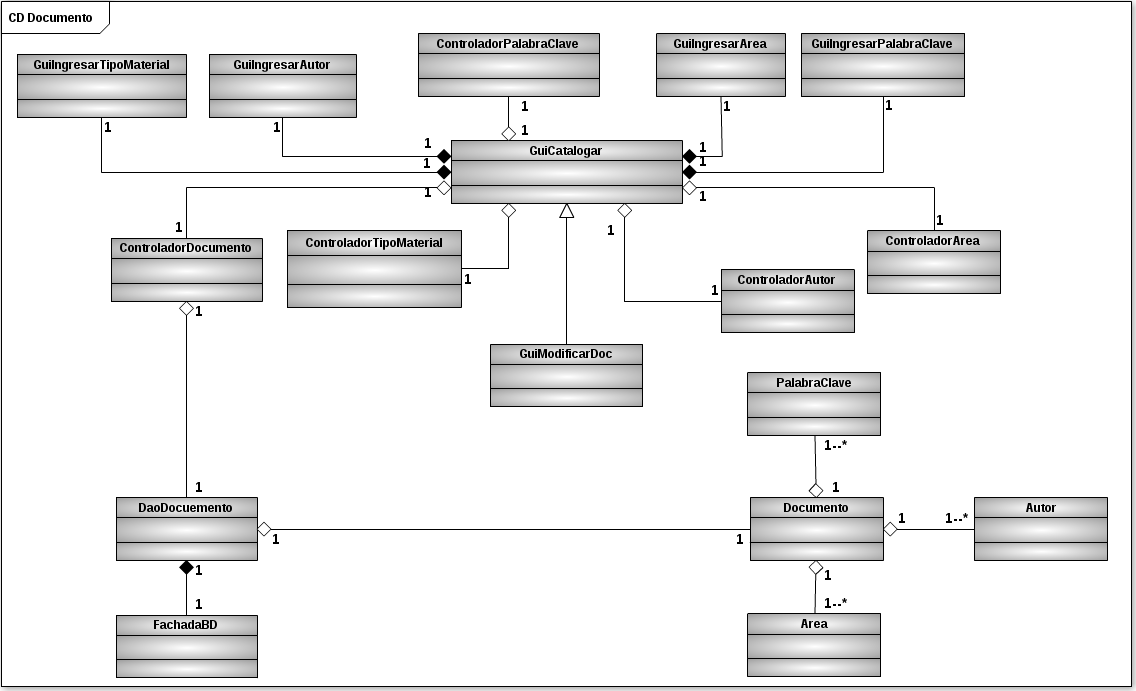
\includegraphics[width=20cm, height=17cm, angle=90]{diagramasClase/DiagramaClases2}
	\end{minipage}
			
	%especificación detallada
	%\documentclass{article}
%
%\usepackage[spanish]{babel}
%\usepackage[utf8]{inputenc}
%\usepackage{geometry}
%\usepackage{graphicx}
%\geometry{tmargin=3cm,bmargin=3cm,lmargin=3cm,rmargin=2cm}
%
%\begin{document}

\setlength{\unitlength}{1cm}
%\begin{picture}(17,21)
%\put(0,0) {\line(1,0){17}}
%\put(0,21) {\line(1,0){17}}
%\put(0,21) {\line(0,-1){21}}
%\put(17,21) {\line(0,-1){21}}
%\end{picture}

\begin{picture}(17,21)
\put(8,4)
{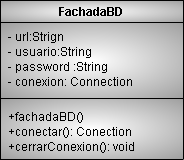
\includegraphics[width=5cm, height=4cm]{DiagramasClase/Utilidades}}
\put(0,0)
{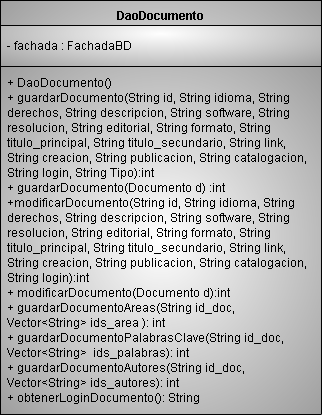
\includegraphics[width=7cm, height=10cm]{DiagramasClase/Documentos/DaoDocumento}}
\put(4,11)
{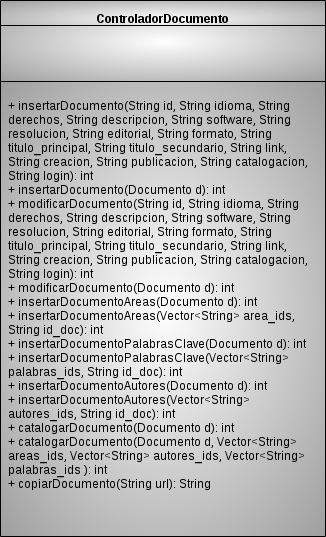
\includegraphics[width=7cm, height=10cm]{DiagramasClase/Documentos/ControladorDocumento}}
\end{picture}


\newpage

\begin{picture}(17,21)
\put(0,0)
{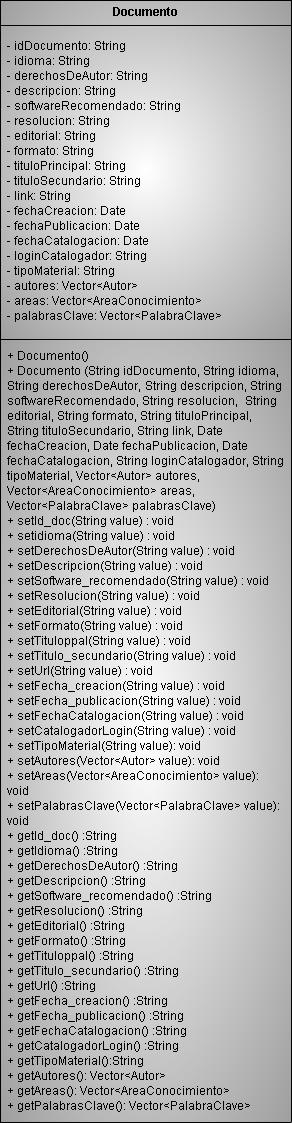
\includegraphics[width=7cm, height=21cm]{DiagramasClase/Documentos/Documento}}
\put(8,-1)
{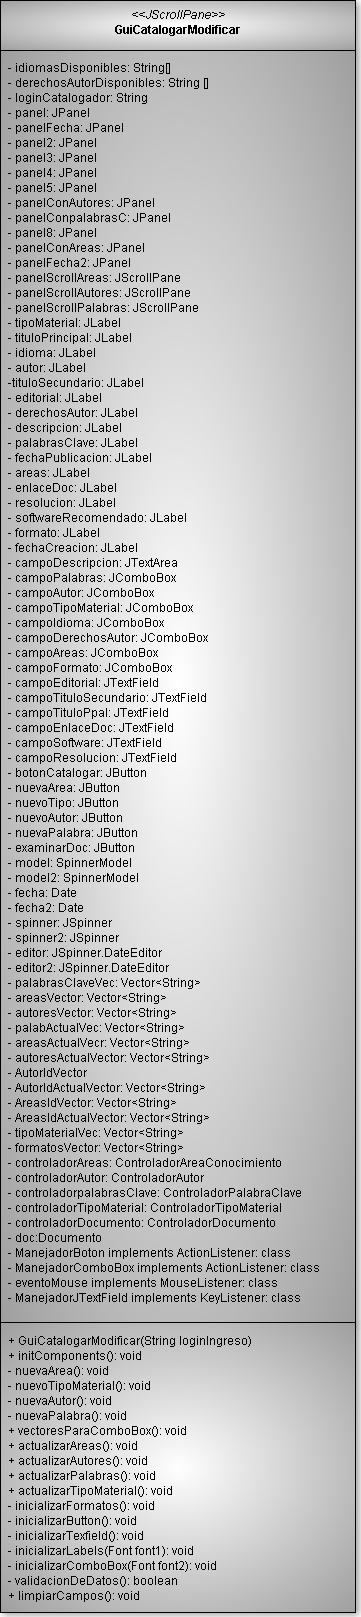
\includegraphics[width=8cm, height=22cm]{DiagramasClase/Documentos/GuiCatalogarModificar}}
\end{picture}

%\end{document}	
			
	%-------------------------------------------------------------------------------	
	
			
	\begin{tabular}{|p{5cm}|p{11cm}|}\hline
	{\bf Titulo} & {Diagrama de Clases Consulta}\\
	\hline
	{\bf Descripción} & {El diagrama de clases consulta reúne todas las clases
	relacionadas con las consultas a documentos que los usuario realizan en el sistema,
	ya sean consultas generales o avanzadas. Para esto se tiene las clases que interactúan
	directamente con el usuario como lo son: GuiVistaDocumento que permite ver la información del
	documento de forma detallada, GuiConsultaBasica es la que permite que un usuario del sistema
	pueda realizar una consulta de forma rápida, GuiConsultaAvanzada que permite realizar una
	búsqueda introduciendo datos específicos y la clase GuiResultadoConsulta que es la que permite
	ver la lista de documentos que se encuentran después de realizar una consulta usando ya sea
	GuiConsultaBasica o GuiConsultaAvanzada.\newline
	También se incluyen las clases ControladorConsulta que realiza verificaciones sobre los
	parámetros de búsqueda de una consulta y envía los respectivos valores a la clase DaoConsulta
	la cual realiza la consulta a la base de datos del sistema y construye la respuesta. Y se usar
	la clase FachadaBD para lograr la conexión con la base de datos.}\\
	\hline
	\end{tabular}\\[.5cm]
		
	\begin{tabular}{|p{3.5cm}|p{4.5cm}|p{2.5cm}|p{4.5cm}|}\hline
	{\bf Creado Por} & {María Andrea Cruz} & {\bf Fecha} & {Abril 27 2011}\\
	\hline
	{\bf Actualizado por} & {Yerminson Gonzalez} & {\bf Fecha} & {Mayo 11 2011}\\
	\hline
	\end{tabular}

	\begin{minipage}[c]{1\linewidth}
	\centering
	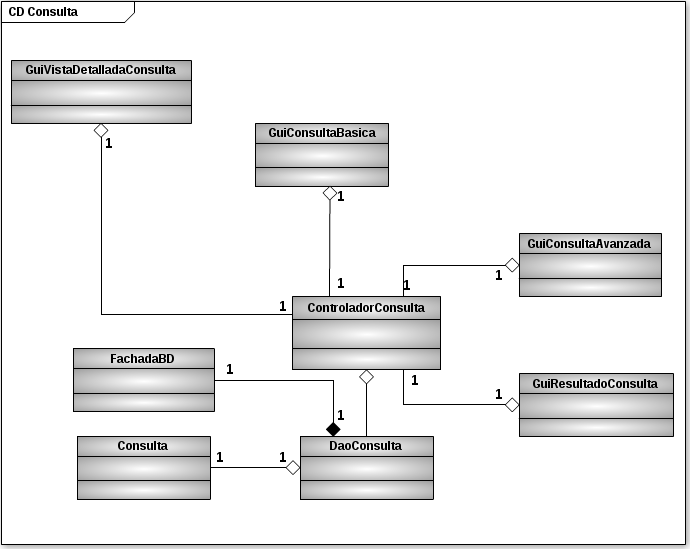
\includegraphics[width=20cm, height=17cm, angle=90]{diagramasClase/DiagramaClases3}
	\end{minipage}
			
	%especificación detallada
	%\documentclass{article}
%
%\usepackage[spanish]{babel}
%\usepackage[utf8]{inputenc}
%\usepackage{geometry}
%\usepackage{graphicx}
%\geometry{tmargin=3cm,bmargin=3cm,lmargin=3cm,rmargin=2cm}
%
%\begin{document}
\setlength{\unitlength}{1cm}

\begin{picture}(17,21)
\put(0,16)
{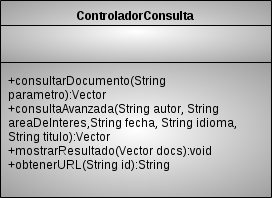
\includegraphics[width=7cm, height=5cm]{DiagramasClase/Consultas/ControladorConsulta}}
\put(7.5,16)
{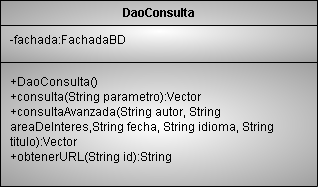
\includegraphics[width=7cm, height=5cm]{DiagramasClase/Consultas/DaoConsulta}}
\put(0,11,5)
{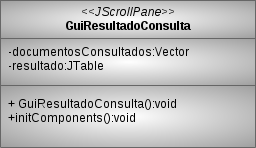
\includegraphics[width=7cm, height=4cm]{DiagramasClase/Consultas/GuiResultadoConsulta}}
\put(7.5,10.5)
{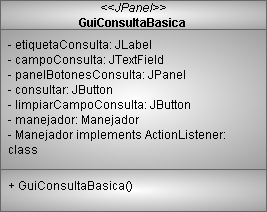
\includegraphics[width=7cm, height=5cm]{DiagramasClase/Consultas/GuiConsultaBasica}}
\put(0,-1)
{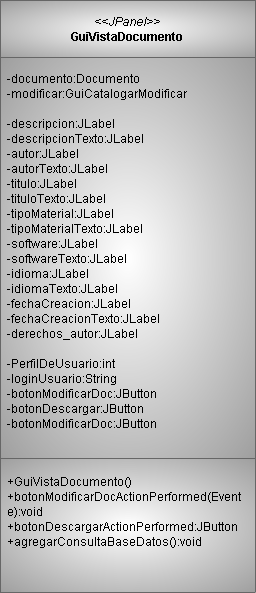
\includegraphics[width=7cm, height=12cm]{DiagramasClase/Consultas/GuiVistaDocumento}}
\put(7.5,0)
{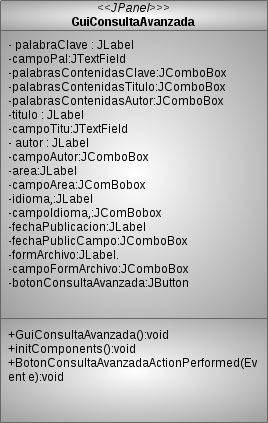
\includegraphics[width=7cm, height=10cm]{DiagramasClase/Consultas/GuiConsultaAvanzada}}
\end{picture}

%\end{document}
			
	%-------------------------------------------------------------------------------			
	
		
	\begin{tabular}{|p{5cm}|p{11cm}|}\hline
	{\bf Titulo} & {Diagrama de Clases Reporte}\\
	\hline
	{\bf Descripción} & {El diagrama de clases reporte reúne todas las clases
	relacionadas con la generación de reportes del sistema para observar estadísticas y
	comportamientos de los usuarios del sistema.\newline
	Se incluyen las clases GuiReportes que permite al usuario administrador escoger de manera
	parametrizada las variables para generar el reporte, ControladorReportes realiza
	verificaciones y envía a la clase DaoReportes quien es la clase que realiza las consultas a
	la base de datos del sistema. La clase FachadaBD es usada para realizar la conexión a la
	base de datos.}\\
	\hline
	\end{tabular}\\[.5cm]
		
	\begin{tabular}{|p{3.5cm}|p{4.5cm}|p{2.5cm}|p{4.5cm}|}\hline
	{\bf Creado Por} & {Yerminson Gonzalez} & {\bf Fecha} & {Abril 28 2011}\\
	\hline
	{\bf Actualizado por} & {María Andrea Cruz} & {\bf Fecha} & {Mayo 11 2011}\\
	\hline
	\end{tabular}\\[.5cm]

	\begin{minipage}[c]{1\linewidth}
	\centering
	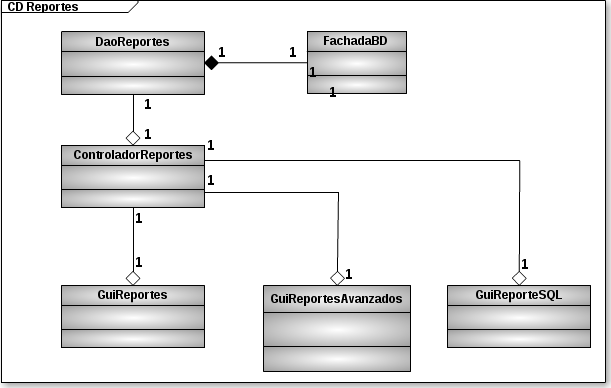
\includegraphics[width=13cm, height=12cm]{diagramasClase/DiagramaClases4}
	\end{minipage}
			
	%especificación detallada
	%\documentclass{article}
%
%\usepackage[spanish]{babel}
%\usepackage[utf8]{inputenc}
%\usepackage{geometry}
%\usepackage{graphicx}
%\geometry{tmargin=3cm,bmargin=3cm,lmargin=3cm,rmargin=2cm}
%
%\begin{document}
\setlength{\unitlength}{1cm}

\begin{picture}(17,21)
\put(1,17)
{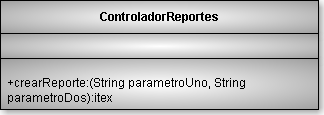
\includegraphics[width=5cm, height=4cm]{DiagramasClase/Reportes/ControladorReportes}}
\put(1,9)
{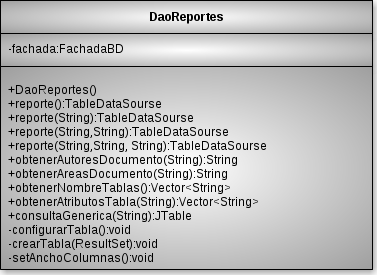
\includegraphics[width=5cm, height=7cm]{DiagramasClase/Reportes/DaoReportes}}
\put(7,11)
{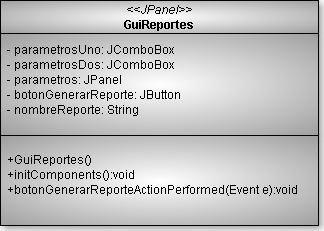
\includegraphics[width=6cm, height=10cm]{DiagramasClase/Reportes/GuiReportes}}
\put(1,0)
{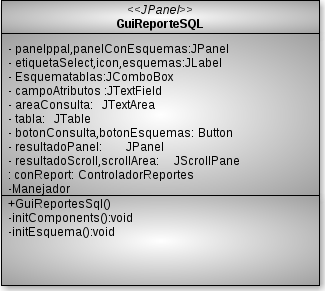
\includegraphics[width=5cm, height=8cm]{DiagramasClase/Reportes/GuiReporteSQL}}
\put(7,-1)
{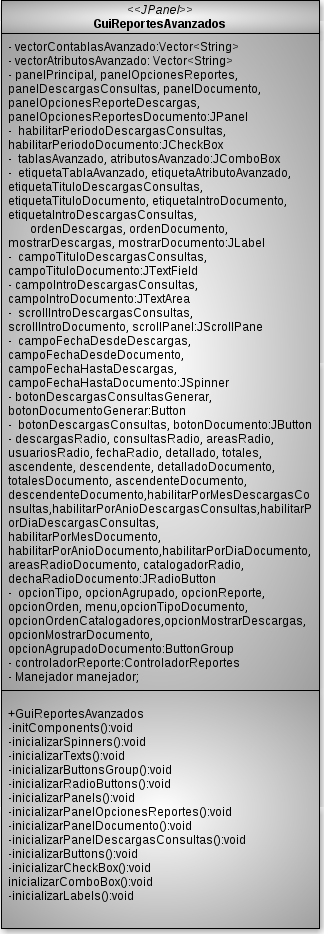
\includegraphics[width=6cm, height=11cm]{DiagramasClase/Reportes/GuiReportesAvanzados}}
\end{picture}

%\end{document}		

	%-------------------------------------------------------------------------------			

		
	\begin{tabular}{|p{5cm}|p{11cm}|}\hline
	{\bf Titulo} & {Diagrama de Clases Gestión Documentos}\\
	\hline
	{\bf Descripción} & {El diagrama de clases gestión documentos reúne todas las
	clases relacionadas con la catalogación de documentos en el sistema.\newline
	Se tiene las clases GuiIngresarArea, GuiIngresarAutor, GuiIngresarTipoMaterial, 
	GuiIngresarPalabraClave que son las interfaces que permiten al usuario con perfil
	catalogador o administrador ingresar nuevas áreas, autores, tipos de material y palabras
	clave.\newline
	Las clases ControladorArea, ControladorAutor, ControladorTipoMaterial, ControladorPalabraClave
	son las clases que permiten verificar que los datos ingresados por el usuario están bien 
	diligenciados y que se pueden ingresar al sistema. Las clases DaoAutor, DaoAreaConocimiento,
	DaoTipoMaterial, y DaoPalabraClave son las clases que interactúan directamente con la 
	base de datos y permite el ingreso de estos datos al sistema. La clase FachadaBD se usa
	para crear la conexión con la base de datos.\newline
	Finalmente las clases AreaConocimiento, Autor, TipoMaterial, PalabraClave modelan las entidades
	Area, Autor, TipoMaterial, PalabraClave respectivamente del modelo de datos planteado, y se 
	usan de las guis hacia abajo.}\\
	\hline
	\end{tabular}\\[.5cm]
		
	\begin{tabular}{|p{3.5cm}|p{4.5cm}|p{2.5cm}|p{4.5cm}|}\hline
	{\bf Creado Por} & {Edgar Andrés Moncada} & {\bf Fecha} & {Abril 28 2011}\\
	\hline
	{\bf Actualizado por} & {María Andrea Cruz} & {\bf Fecha} & {Mayo 11 2011}\\
	\hline
	\end{tabular}

	\begin{minipage}[c]{1\linewidth}
	\centering
	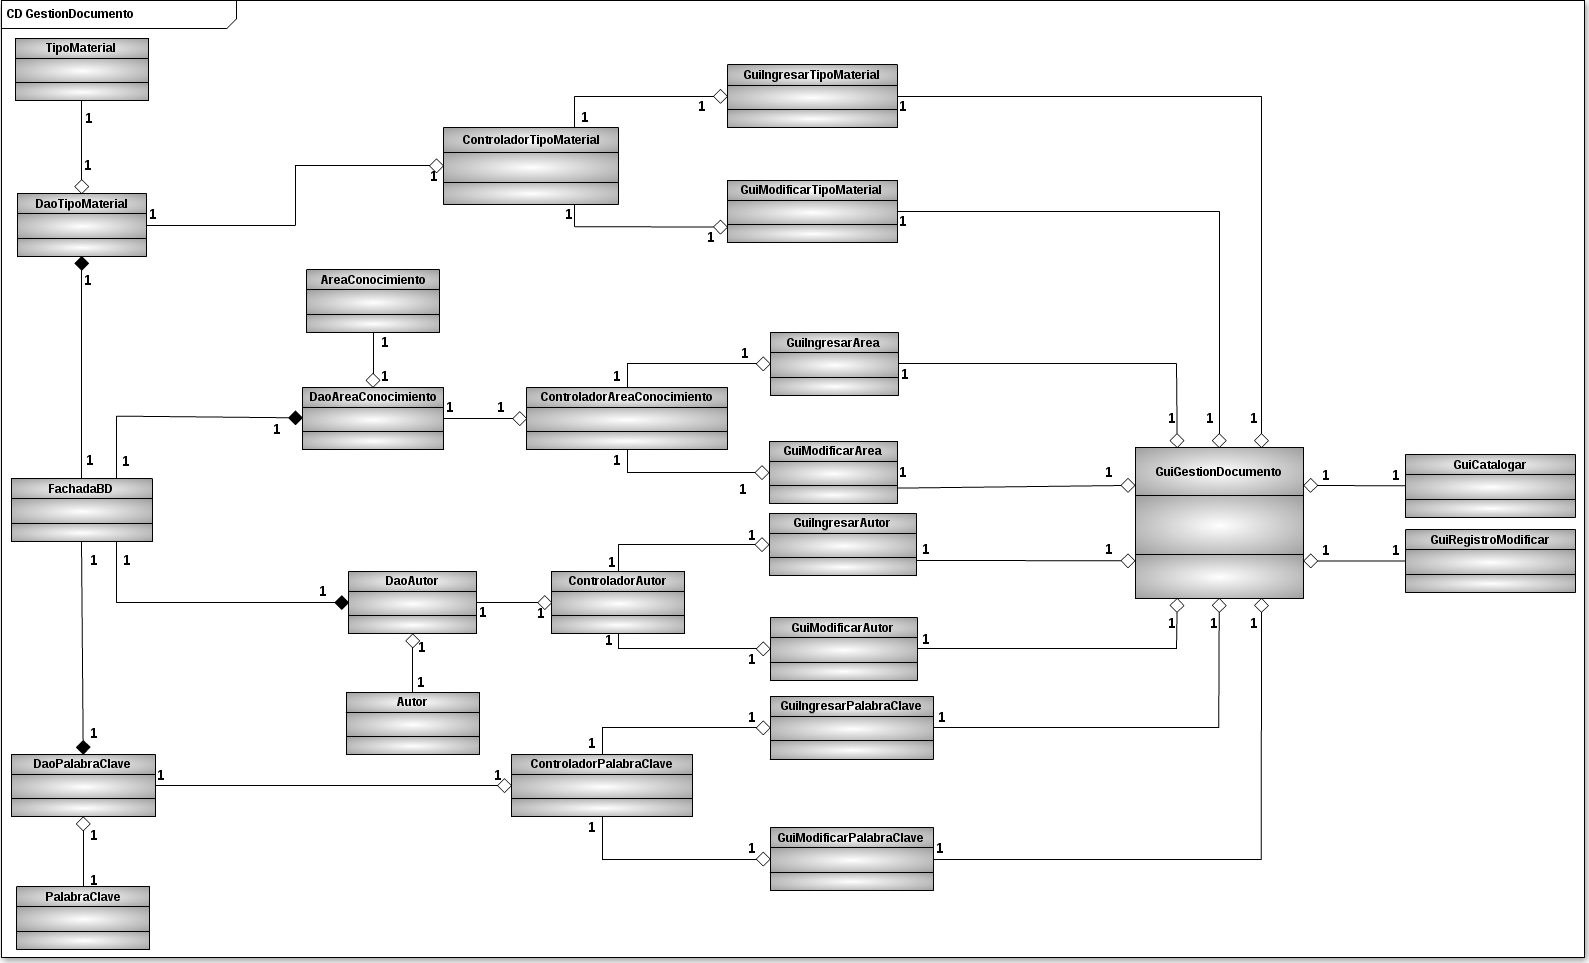
\includegraphics[width=21cm, height=17cm, angle=90]{diagramasClase/DiagramaClases5}
	\end{minipage}
			
	%especificación detallada
	%\documentclass{article}
%
%\usepackage[spanish]{babel}
%\usepackage[utf8]{inputenc}
%\usepackage{geometry}
%\usepackage{graphicx}
%\geometry{tmargin=3cm,bmargin=3cm,lmargin=3cm,rmargin=2cm}
%
%\begin{document}
\setlength{\unitlength}{1cm}

\begin{picture}(17,21)
\put(0,1)
{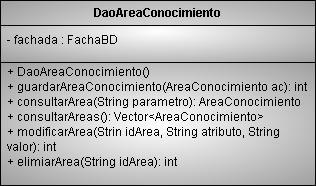
\includegraphics[width=6cm, height=5cm]{DiagramasClase/GestionDocumento/DaoAreaConocimiento}}
\put(0,7)
{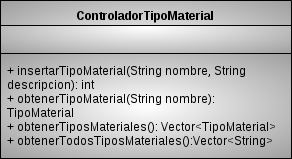
\includegraphics[width=6cm, height=4cm]{DiagramasClase/GestionDocumento/ControladorTipoMaterial}}
\put(0,12)
{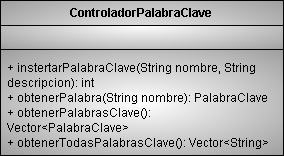
\includegraphics[width=6cm, height=4cm]{DiagramasClase/GestionDocumento/ControladorPalabraClave}}
\put(0,17)
{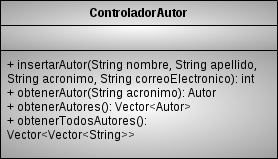
\includegraphics[width=6cm, height=4cm]{DiagramasClase/GestionDocumento/ControladorAutor}}
\put(7,12)
{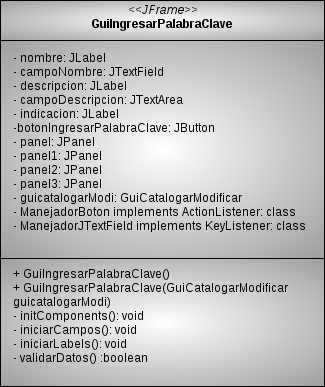
\includegraphics[width=7cm, height=9cm]{DiagramasClase/GestionDocumento/GuiIngresarPalabraClave}}
\put(7,2)
{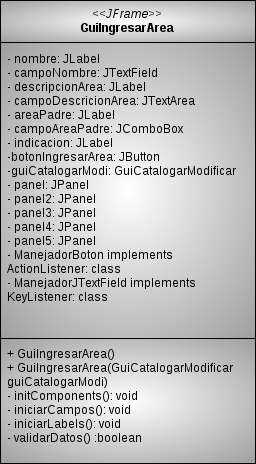
\includegraphics[width=6cm, height=9cm]{DiagramasClase/GestionDocumento/GuiIngresarArea}}
\end{picture}

\newpage

\begin{picture}(17,21)
\put(0,12)
{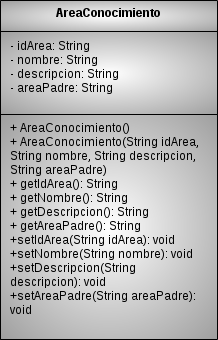
\includegraphics[width=6cm, height=9cm]{DiagramasClase/GestionDocumento/AreaConocimiento}}
\put(0,0)
{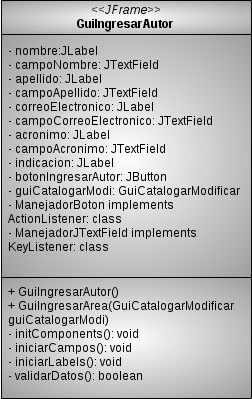
\includegraphics[width=6cm, height=10cm]{DiagramasClase/GestionDocumento/GuiIngresarAutor}}
\put(7,10)
{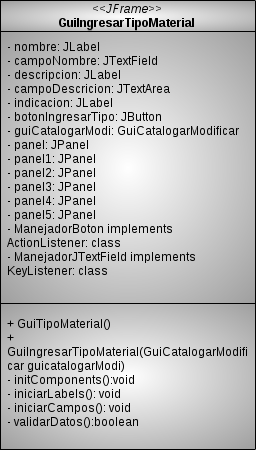
\includegraphics[width=6cm, height=11cm]{DiagramasClase/GestionDocumento/GuiIngresarTipoMaterial}}
\put(7,0)
{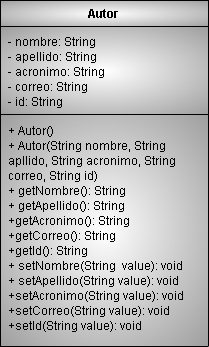
\includegraphics[width=6cm, height=9cm]{DiagramasClase/GestionDocumento/Autor}}
\end{picture}

\newpage

\begin{picture}(17,21)
\put(0,17)
{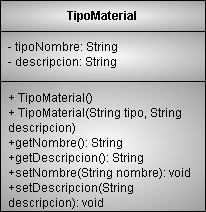
\includegraphics[width=5cm, height=5cm]{DiagramasClase/GestionDocumento/TipoMaterial}}
\put(0,10)
{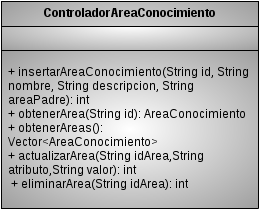
\includegraphics[width=6cm, height=6cm]{DiagramasClase/GestionDocumento/ControladorAreaConocimiento}}
\put(0,5)
{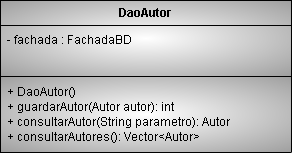
\includegraphics[width=5cm, height=4cm]{DiagramasClase/GestionDocumento/DaoAutor}}
\put(6,17)
{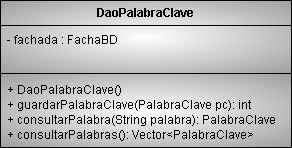
\includegraphics[width=6cm, height=5cm]{DiagramasClase/GestionDocumento/DaoPalabraClave}}
\put(7,12)
{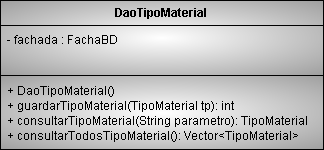
\includegraphics[width=6cm, height=4cm]{DiagramasClase/GestionDocumento/DaoTipoMaterial}}
\put(7,7)
{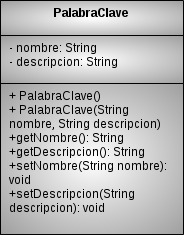
\includegraphics[width=4cm, height=4cm]{DiagramasClase/GestionDocumento/PalabraClave}}
\end{picture}


%\end{document}	
			
	%-------------------------------------------------------------------------------		
			
	\begin{tabular}{|p{5cm}|p{11cm}|}\hline
	{\bf Titulo} & {Diagrama de Clases Principal}\\
	\hline
	{\bf Descripción} & {El diagrama de clases principal reúne todas las clases que le
	dan forma al sistema, es decir, las interfaces gráficas mediante las cuales los
	usuarios finales podrán interactuar con el sistema.\newline
	Se incluyen las clases GuiPrincipla que es la interfaz que un usuario del sistema
	verá en primera medida, permite realizar consultar, registrarse en el sistema e ingresar al
	sistema, GuiAdministrador que es la interfaz que contiene las opciones para el administrador,
	GuiCatalogador es la interfaz para el usuario con perfil catalogador, contiene las opciones 
	para catalogar documentos, GuiUsuarioNormal que es la interfaz que en principio tiene un 
	usuario recien registrado al sistema y la clase ControladorVentanaPrincipal que es la clase
	que realiza el manejo de las guis, y la verificación de un usuario que quiere ingresar al
	sistema.\newline
	Las clases GuiConsultarUsuarios, GuiAutenticar, GuiRegistroModificar, GuiCatalogarModificar,
	GuiConsultaBasica, GuiConsultaAvanzada, y Usuario se usan para lograr las interfaces 
	finales.}\\
	\hline
	\end{tabular}\\[.5cm]
				
	\begin{tabular}{|p{3.5cm}|p{4.5cm}|p{2.5cm}|p{4.5cm}|}\hline
	{\bf Creado Por} & {Luis Felipe Vargas} & {\bf Fecha} & {Abril 28 2011}\\
	\hline
	{\bf Actualizado por} & {Yerminson Gonzalez} & {\bf Fecha} & {Mayo 11 2011}\\
	\hline
	\end{tabular}
	
	\begin{minipage}[c]{1\linewidth}
	\centering
	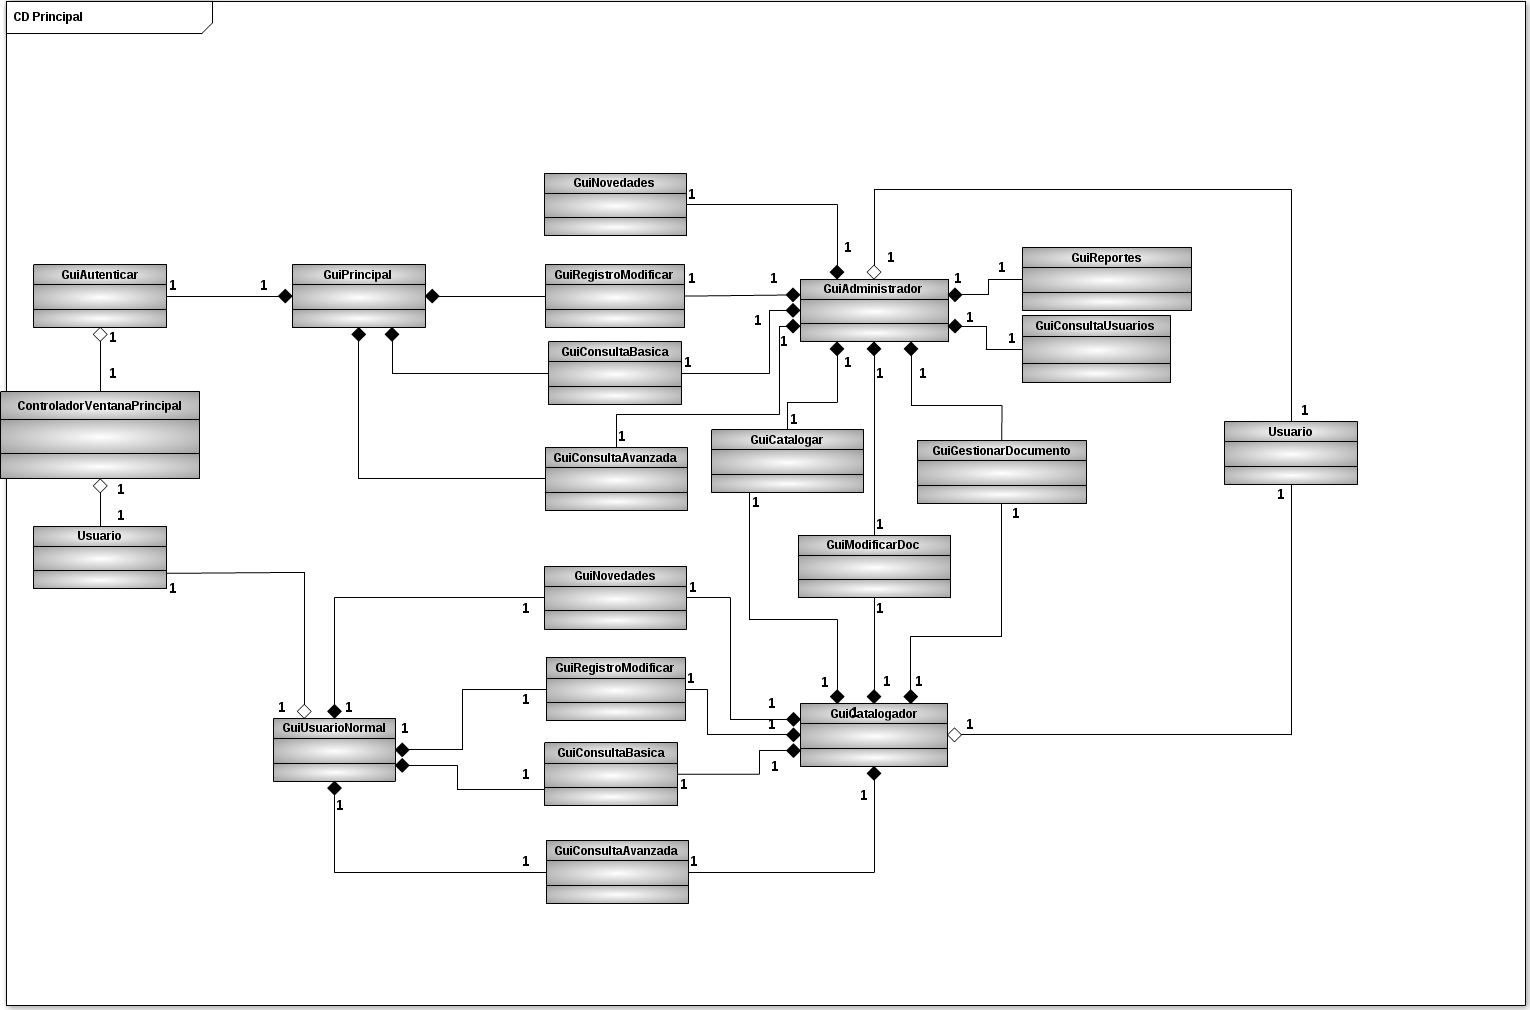
\includegraphics[width=20cm, height=17cm, angle=90]{diagramasClase/DiagramaClases6}
	\end{minipage}
			
	%especificación detallada
	%\documentclass{article}
%
%\usepackage[spanish]{babel}
%\usepackage[utf8]{inputenc}
%\usepackage{geometry}
%\usepackage{graphicx}
%\geometry{tmargin=3cm,bmargin=3cm,lmargin=3cm,rmargin=2cm}
%
%\begin{document}
\setlength{\unitlength}{1cm}

\begin{picture}(17,21)
\put(0,15)
{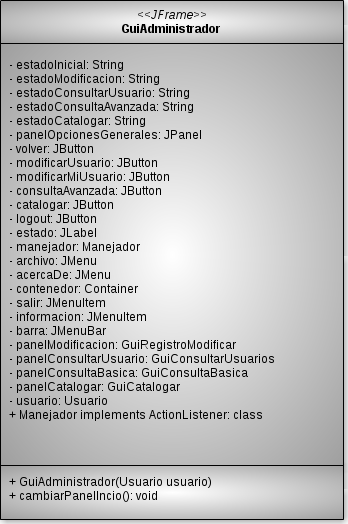
\includegraphics[width=6cm, height=10cm, angle=90]{DiagramasClase/Principal/GuiAdministrador}}
\put(0,8)
{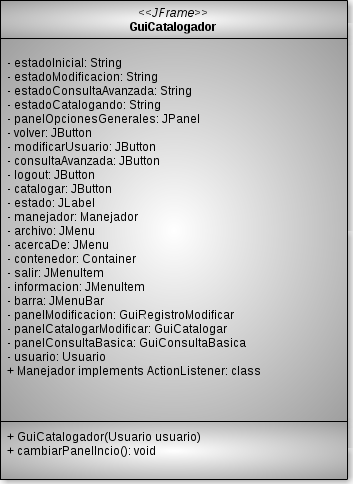
\includegraphics[width=6cm, height=10cm, angle=90]{DiagramasClase/Principal/GuiCatalogador}}
\put(0,1)
{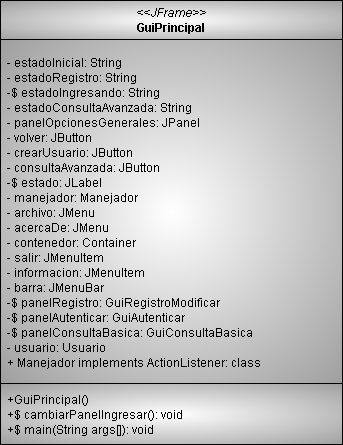
\includegraphics[width=6cm, height=10cm, angle=90]{DiagramasClase/Principal/GuiPrincipal}}
\put(10.5,11)
{\includegraphics[width=6.5cm, height=10cm]{DiagramasClase/Principal/GuiUsuarioNormal}}
\put(10.5,1)
{\includegraphics[width=8cm, height=4cm, angle=90]{DiagramasClase/Principal/ControladorVentanaPrincipal}}

\end{picture}

%\end{document}	
	
	%-------------------------------------------------------------------------------
	
\subsection{Modelo ER} 
	\begin{minipage}[c]{1\linewidth}
	    \centering
        \includegraphics[width=19cm, height=17cm, angle=90]{modeloDatos}
    \end{minipage}\\[.1cm]
       	
    \begin{tabular}{|p{3.5cm}|p{4.5cm}|p{2.5cm}|p{4.5cm}|}\hline
	{\bf Creado Por} & {Yerminson Gonzalez} & {\bf Fecha} & {Abril 28 2011}\\
	\hline
	{\bf Actualizado por} & {Yerminson Gonzalez} & {\bf Fecha} & {Mayo 15 2011}\\
	\hline
	{\bf Actualizado por} & {Yerminson Gonzalez} & {\bf Fecha} & {Mayo 29 2011}\\
	\hline
	\end{tabular}
        	
\subsection{Diagrama de Paquetes}
	\begin{minipage}[c]{1\linewidth}
	    \centering
        \includegraphics[width=19.5cm, height=17cm, angle=90]{diagramaPaquetes}
    \end{minipage}\\[.3cm]
       	
    \begin{tabular}{|p{3.5cm}|p{4.5cm}|p{2.5cm}|p{4.5cm}|}\hline
	{\bf Creado Por} & {Edgar Moncada} & {\bf Fecha} & {Mayo 14 2011}\\
	\hline
	{\bf Actualizado por} & {Edgar Moncada} & {\bf Fecha} & {Junio 7 2011}\\
	\hline
	\end{tabular}
	
\subsection{Prototipos de Interfaz de Usuario}
%\documentclass[]{article}
%\usepackage[utf8]{inputenc}
%\usepackage[]{graphicx}
%\usepackage{geometry}
%
%\begin{document}

\begin{minipage}[c]{1\textwidth}
	\begin{center}
	\includegraphics[width= 10cm , height= 5cm]{prototiposGui/AUTENTICAR}
	\end{center}
	{Prototipo de interfaz {\bf Autenticar Usuario} , la cual permite ingresar al sistema como
	usuario con ciertos privilegios.}
\end{minipage}\\[1cm]

\begin{minipage}[c]{1\textwidth}
	\begin{center}
	\includegraphics[width= 10cm , height= 5cm,]{prototiposGui/consultarUsuarios}
	\end{center}
	{Prototipo de interfaz {\bf Consultar Usuarios} la cual permite al administrador consultar los
	usuarios de la base de datos y modificar algunos datos de estos.}
\end{minipage}\\[1cm]

\begin{minipage}{1\textwidth}
	\begin{center}
	\includegraphics[width= 20cm , height= 13cm,angle=90]{prototiposGui/guiPpal}
	\end{center}
	{Prototipo de la {\bf Interfaz de Inicio}, la cual varia en su sección B de acuerdo al perfil
	del usuario actualmente autentificado siendo seccion B.1 usuario administrador  , seccion B.2
	usuario catalogardor y seccion B.3 usuario normal.}
\end{minipage}\\[1cm]


\begin{minipage}{1\textwidth}
	\begin{center}
	\includegraphics[width= 17cm , height= 15cm]{prototiposGui/catalogarDoc}
	\end{center}
	{Prototipo de la interfaz {\bf Catalogar Documento} la cual permite añadir nuevos documento a
	la base de datos con ciertos metadatos ya especificados.}
\end{minipage}

\begin{minipage}{1\textwidth}
	\begin{center}
	\includegraphics[width= 17cm , height= 13cm]{prototiposGui/registro}
	\end{center}
	{Prototipo de la interfaz {\bf Registro de Usuarios} mediante la cual ingresa sus datos el
	usuario para pertenecer al sistema. }
\end{minipage}

\begin{minipage}{1\textwidth}
	\begin{center}
	\includegraphics[width= 17cm , height= 13cm]{prototiposGui/modificarUsuarios}
	\end{center}
	{Prototipo de la interfaz {\bf Modificar Datos de Usuarios} la cual me permite modificar solo
	algunos	datos del usuario activo. }
\end{minipage}

\begin{minipage}{1\textwidth}
	\begin{center}
	\includegraphics[width= 17cm , height= 13cm]{prototiposGui/gestionDocumento.JPG}
	\end{center}
	{Prototipo de las interfaces que tiene que ver con la {\bf Gestión de Documento}; Ingresar un
	nuevo autor, una nueva palabra clave, un nuevo tipo material y una nueva área a la que
	pertenece el documento. }
\end{minipage}

%\end{document}

\subsection{Diagrama de Despliegue}
\begin{minipage}{1\textwidth}
	\centering
	\includegraphics[scale=0.8]{diagramaDespliegue}
\end{minipage}\\[1cm]

%\end{document}